% !Mode:: "TeX:UTF-8"

%%%%%%% 正文 %%%%%%%

\chapter{一个测试}

\section{真的只是一个测试}

中文学位论文测试。

\subsection{测试}

一只敏捷的棕色狐狸跳过那只懒惰的狗。

\chapter{继续测试}

\section{测试}

由公式

\[E = mc^2\]

\noindent 下面列出了一些应采用直立数学字体的数学常数和数学符号。

\vspace{-0.5em}
\begin{center}
\begin{tabularx}{0.7\textwidth}{XX}
$\mathrm{d}$、 $\mathrm{D}$、 $\mathrm{p}$~———微分算子 & $\mathrm{e}$~———自然对数之底数 \\
$\mathrm{i}$、 $\mathrm{j}$~———虚数单位 & $\piup$———圆周率\\
\end{tabularx}
\end{center}

\section{行内公式}

出现在正文一行之内的公式称为行内公式,例如~$f(x)=\int_{a}^{b}\frac{\sin{x}}{x}\mathrm{d}x$。对于非矩阵和非多行形式的行内公式,一般不会使得行距发生变化,而~Word~等软件却会根据行内公式的竖直距离而自动调节行距,如图~\ref{fig:hangju}~所示。

\begin{figure}[htbp]
\centering
\subfigure[由~\LaTeX~系统生成的行内公式]{\label{fig:subfig:latex}
                \fbox{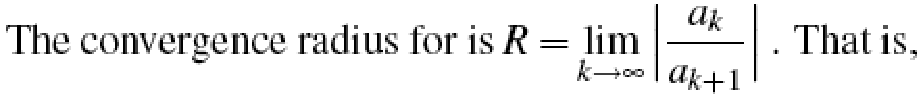
\includegraphics[width=0.55\textwidth]{latex}}}
\subfigure[由~Word软件生成的~.doc~格式行内公式]{\label{fig:subfig:word}
                \fbox{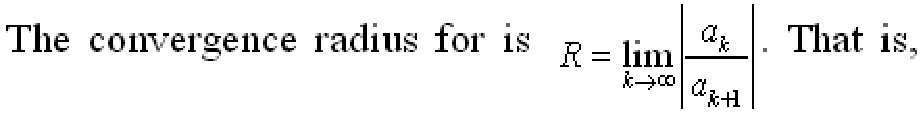
\includegraphics[width=0.55\textwidth]{word}}}
\subfigure[由~Word软件生成的~.pdf~格式行内公式]{\label{fig:subfig:pdf}
                \fbox{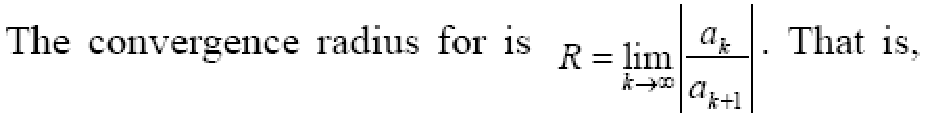
\includegraphics[width=0.55\textwidth]{pdf}}}

\caption{由~\LaTeX~和~Word~生成的~3~种行内公式屏显效果}\label{fig:hangju}
\vspace{-1em}
\end{figure}

\section{代码环境}

很多和计算机专业背景相关的同学都会使用到代码环境,使用~\verb|\verb|~指令或者是~\verb|verbatim|~环境固然是一种选择,但是比不上专门的~lstlisting~环境这么专业。

\begin{lstlisting}
int main(int argc, char ** argv) {
    printf("Hello world!\n");
    return 0;
}
\end{lstlisting}

\noindent\hrule
\vspace{0.1em}\noindent\hrule

\vspace{1em}

\section{普通表格的绘制方法}

表格应具有三线表格式,因此需要调用~booktabs~宏包,其标准格式如表 \ref{tab:table1} 所示。
\begin{table}[htbp]
\caption{符合本科生毕业论文绘图规范的表格}\label{tab:table1}
\vspace{0.5em}\centering\wuhao
\begin{tabular}{ccccc}
\toprule[1.5pt]
$D$(in) & $P_u$(lbs) & $u_u$(in) & $\beta$ & $G_f$(psi.in)\\
\midrule[1pt]
 5 & 269.8 & 0.000674 & 1.79 & 0.04089\\
10 & 421.0 & 0.001035 & 3.59 & 0.04089\\
20 & 640.2 & 0.001565 & 7.18 & 0.04089\\
 5 & 269.8 & 0.000674 & 1.79 & 0.04089\\
10 & 421.0 & 0.001035 & 3.59 & 0.04089\\
20 & 640.2 & 0.001565 & 7.18 & 0.04089\\
 5 & 269.8 & 0.000674 & 1.79 & 0.04089\\
10 & 421.0 & 0.001035 & 3.59 & 0.04089\\
20 & 640.2 & 0.001565 & 7.18 & 0.04089\\
 5 & 269.8 & 0.000674 & 1.79 & 0.04089\\
10 & 421.0 & 0.001035 & 3.59 & 0.04089\\
20 & 640.2 & 0.001565 & 7.18 & 0.04089\\
\bottomrule[1.5pt]
\end{tabular}
\vspace{\baselineskip}
\end{table}

就是这样。

%%%%%%% 结论 %%%%%%%

\addcontentsline{toc}{chapter}{结\quad 论} %添加到目录中

\chapter*{结\quad 论}

得出结论,楼主傻逼。